%%
%% Author: Thomas Schouten
%% 05-03-2018
%%

% Preamble
\documentclass[border=5mm, tikz]{standalone}

\usepackage{tikz}

\usetikzlibrary{positioning, arrows.meta, shapes.geometric}


% Default arrow length: (length right, length up)
\newcommand{\stdlength}{1,0}

% Default arrowhead.
\newcommand{\stdarrow}{-{Latex[length=2mm,width=2mm]}}

% Document
\begin{document}

    
\begin{tikzpicture}
        \node[left] (one) { One };
        \draw[\stdarrow] (one.east) -- ++(\stdlength)
        node[right] (two) { Twoooooooooooooo };
        \draw[\stdarrow] (two.east) -- ++(\stdlength)
        node[right] (three) { Three };
        \draw[\stdarrow] (three.east) -- ++(\stdlength)
        node[right] (four) { Four };
    \end{tikzpicture}

    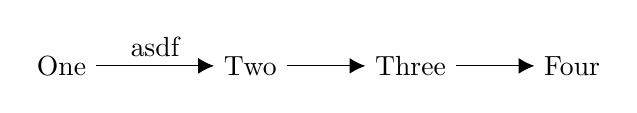
\begin{tikzpicture}
        \node[left] (one) { One };
        \draw[\stdarrow] (one.east) -- ++(1.5,0)  node[above, pos=0.5] { asdf }
        node[right] (two) { Two };
        \draw[\stdarrow] (two.east) -- ++(\stdlength)
        node[right] (three) { Three };
        \draw[\stdarrow] (three.east) -- ++(\stdlength)
        node[right] (four) { Four };
    \end{tikzpicture}

    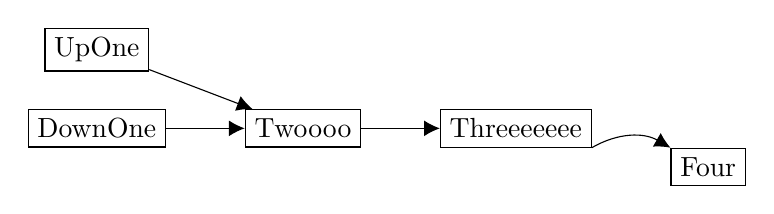
\begin{tikzpicture}[every node/.style={shape=rectangle, draw}]
        \node (one) { UpOne };
        \node[below of=one] (two) { DownOne };
        \draw[\stdarrow] (two.east) -- ++(\stdlength)
        node[right] (three) { Twoooo };
        \draw[\stdarrow] (one) -- (three);
        \draw[\stdarrow] (three.east) -- ++(\stdlength)
        node[right] (four) { Threeeeeee };
        \draw[\stdarrow] (four.south east) to [bend left=30] ++(\stdlength)
        node[below right] (five) { Four };
    \end{tikzpicture}

\end{document}